% used for market drawings
\newlength{\slotwidth}
\setlength{\slotwidth}{.103\textwidth}

\section{The Packet-by-Packet Market}
\label{sec:designs}

Our proposal for self-incentivizing networks is a speculative one. To
assess, preliminarily, whether such a scheme could work, we
conducted simulation experiments for a one-hop version of the system.

We describe here the design for a packet-by-packet market that allows
anybody to contribute transmission capacity between two nodes and be
rewarded for it, while endpoints purchase the right to send each
packet, or groups of packets, from the market.

In these systems, the scarce resources of the communications links are
allocated not by TCP, AQM, or a traffic-engineering scheme. Instead,
the links are allocated by a tableau of simultaneous per-timeslice
auctions.

The principal contribution of our findings thus far is that a simple
market-based mechanism, where users bid for the opportunity to send
each packet, can recover schedules that closely approximate the
optimal shortest-remaining-time-first schedule across a contended link.

We discuss here the design for the simple market
(Section~\ref{ss:simplemarket}), our simulation and analytical
evaluation of this system (Section~\ref{ss:eval}), and finally our
unevaluated design for a ``multiresolution'' market that corrects
some of the problems in the simple design.

\subsection{Simple-Market Design}
\label{ss:simplemarket}

\begin{figure*}
\renewcommand{\arraystretch}{2}
\begin{tabular}[height=3in]{|*{8}{p{\slotwidth}|}}
\hline
Time: 0 & Time: 1 & Time: 2 & Time: 3 & Time: 4 & Time: 5 & Time: 6 & Time: 7 \\
\{(A, \$2.01)\} & \{(A, \$2.01)\} & \{(B, )\} & \{(B, )\} & \{(ISP, \$1)\} & \{(ISP, \$1)\} & \{(C, \$10)\} & \{(ISP, \$1)\} \\
\hline
\end{tabular}
\caption{An example snapshot of the ``simple market'' order book. User
A owns the first two time slots and has posted an offer to resel them
for \$2.01 apiece. User B owns the next two slots and has not posted
an offer to sell them. User C owns the slot at time 6 and has posted
an offer of \$10 to sell it. ``ISP'' owns the remaining slots with an offer of \$1 apiece.}
\label{f:simple_market}
\end{figure*}

Our goals for a market were as follows:
\begin{itemize}
\item Let anyone contribute capacity---the ability to transmit a
packet from point A to point B at a certain time.

\item Allow users to act selfishly to maximize their own utility
functions.

\item Allow users to buy, in advance, the right to send packets at a
particular time, which they can then resell. This could be used to
allow a user to construct a virtual link with a certain continuous
throughput.

\item Demonstrate that this system produces a good result globally.
\end{itemize}

Our ``simple'' market is composed of sequential, consecutive time
slots in which a packet can be delivered. Users are able to buy the
right to send a packet within a given time slot.  Once a user buys a slot,
they own a guarantee: if they deliver the packet to one
side of the link by the beginning of the slot, it will make it to the
next hop by the end of the slot interval. The slot owner can also post an offer to re-sell
the slot to another user for a given price.

Figure \ref{f:simple_market} gives an example of the state of the
market's order book---showing the sequential, simultaneous per-timeslice
auctions---at a given time.

The objectives of market users and their flows could vary greatly. In our simulations,
we have experimented with several types, outlined in Figure~\ref{f:user_types}.
\begin{figure*}
\begin{tabular}{|p{.25\textwidth}|p{.70\textwidth}|}
\hline
Flow Type & Objective \\
\hline
\hline
Flow-completion priority & Send $n$ packets, minimizing flow-completion time. \\
\hline
Isochronous flow & Send $n$ packets every $t$ milliseconds. \\
\hline
Deadline flow & Send $n$ packets by deadline $d$. \\
\hline
Evil user & Maximally reduce utility of another market user while
staying within a budget $c$. We discuss the problems of ``evil'' or
strategic bidders in Section~\ref{ss:evil}. \\
\hline
ISP & Simply posts offers to transmit packets; doesn't bid. \\
\hline
\end{tabular}
\caption{Example types of users}
\label{f:user_types}
\end{figure*}

\subsection{Implementation}
We implemented ``bots'' in C++ that participate in the market, placing bids
and offers to maximize the objectives described in Figure~\ref{f:user_types}.

We then built a market simulator, which takes a set of user ``bots''
and executes them in round-robin order, giving them the current order
book and the list of packets actually transmitted on the link (so they
can see which opportunities they have ``won'').

At a given timestep, the simulator runs each bot until all users have
stopped changing the order book, then advances time. When time
advances, any user owns the right to send a packet during front-most
slot in the order book is deemed to send a packet across the link. (If more than one
ISP has offered an opportunity at that slot, more than one packet
might be sent.) The simulation ends when all flows have
completed. We view this as a simplified, idealized model of what might
occur in a home router controlling, e.g., a contended cable-modem link.

\textbf{Flow-completion priority bot:} The implementation of the
``bot'' for flows that care only about their completion time
(``flow-completion priority'' in Figure~\ref{f:user_types} deserves
some further discussion. This type models a flow that arrives at a set time and has a set number of packets $n$ it would like to send as soon as possible. It tries to maximize the utility function $U= -d - c$, where $d$ is the total flow duration and $c$ is the total amount paid for slots.
Upon arrival, this user buys the $n$ slots that maximize its utility function. Once slots have been purchased, it puts up an offer for each slot it owns priced at \$.01 more than negated loss of utility the user would experience if it did not own that slot and had to buy another one.

\subsection{Simple-Market Evaluation}
\label{ss:eval}

\begin{figure}
%\vspace{\baselineskip}
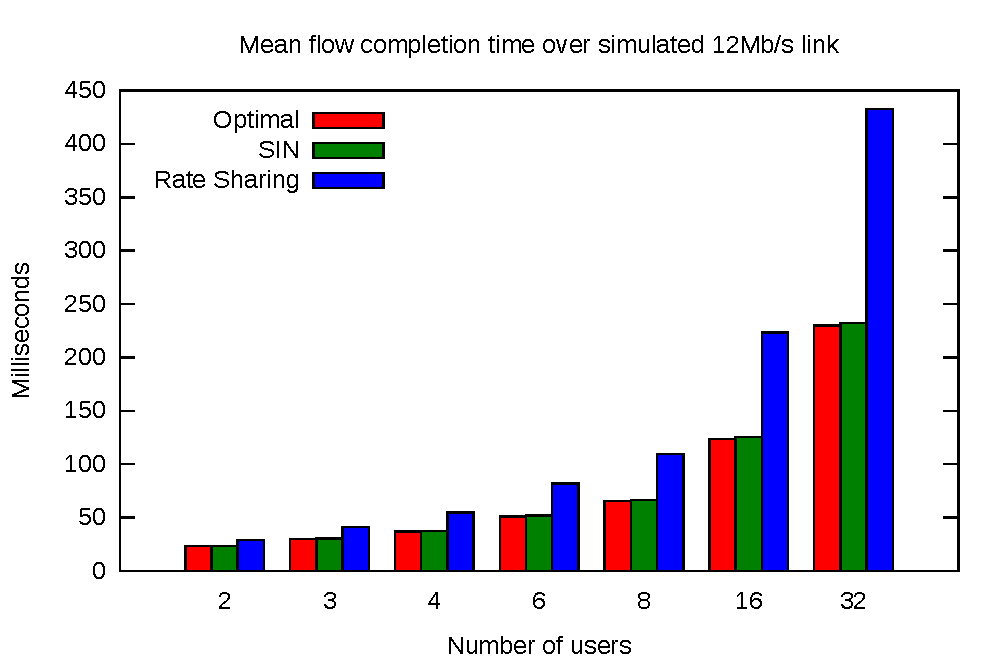
\includegraphics[width=\columnwidth]{plots/delay_over_srtf.pdf}
\caption{Simulation results for 32,000 flows with varying concurrency.}
\label{f:delay_over_srtf}
\end{figure}

\begin{figure}
%\vspace{\baselineskip}
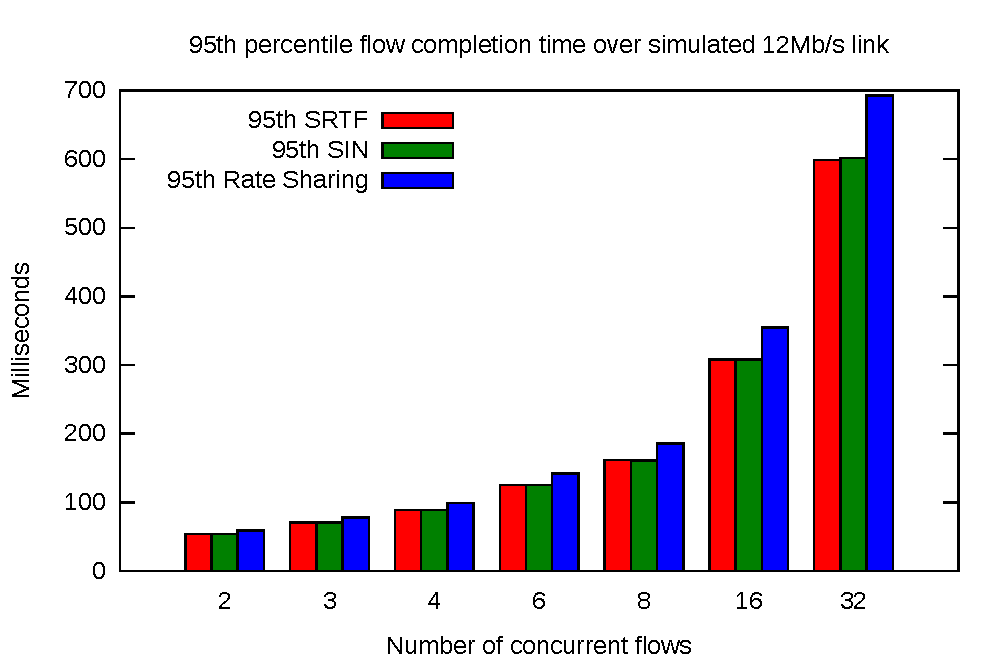
\includegraphics[width=\columnwidth]{plots/95th_delay_over_srtf.pdf}
\caption{95th percentile flow duration.}
\label{f:95th_delay_over_srtf}
\end{figure}

We simulated the results of running a market in practice with flow completion time users that would arrive at time $t$ had a known number of packets $n$ they wanted to send.
Figures~\ref{f:delay_over_srtf} and \ref{f:95th_delay_over_srtf} show the result of running the simulation with 2 to 32 concurrent flow completion time user bots. In this simulation flows arrive at time $uniform(0, 39)$ and have length $uniform(1, 40)$ MTU size packets.
The link being scheduled can send one MTU packet per millisecond (12Mb/s). In the market case, this is manifested by a single owner user that provides 1 packet of capacity every millisecond with an initial offer of \$1 per slot.

We compare the mean flow duration achieved by our market against the shortest remaining time first schedule and an equal rate sharing or round robin schedule. Shortest remaining time first (or SRTF) achieves the minimum possible mean flow duration for an online algorithm with known job durations\cite{karger10,bansal01} (SRTF is also called shortest remaining processing time in some literature).
Rate sharing is an idealized model of what TCP would achieve on FIFO queued router with a large buffer.

As our figures show, the selfish acting bots in our market simulation always converge on a near optimal flow mean flow duration schedule for the link. The majority of time wiht a smaller number of concurrent users, the schedule produced by the market was equivalent to the SRTF schedule. For all numbers of users, the market schedule had mean flow duration that was less than 1\% higher than SRTF.
TODO: talk about 95th chart

\subsubsection{Market Benefits}
SRTF minimizes the mean flow duration but does not attempt to be fair to users. For example, a string of short flows will starve a long flow \cite{bender98}.
Our market recovers solutions equal or close to SRTF in terms of mean flow duration, but it also more fairly distributes value among its users.
If a new flow arrives to a busy market, it must either wait to go after existing flows or directly compensate the owners of the flows it preempts. Like SRTF, a long flow in our market could be starved indefinately by the repeated arrival of short flows, however, this starvation is voluntary by the owner who puts offers up and they would be compensated to infinity to do so.

TODO: it would be cool to have a graph of user utility
\subsubsection{Market Incentives}
Someone who contributes network capacity to the market would be compensated based on the prices they set.
In our current scheme, the market is acting in the interest of its users in sharing the order book and facilitating trades between users.
To incentivize the market to function efficiently, the market could potentially tax every transaction made through it. We will leave further analysis down this path for future work.

\subsubsection{User Disappointment}
Unfortunately, in simulation it is possible that a user bot would have had a higher utility at the end if it refused to put offers on slots it had purchased.
This is possible because our flow completion time user bot bases its offer prices on the offer prices of the slots they would buy instead if their slots are sold, but they are not always able to purchase those replacement slots for those prices (for example if they were sold to someone else who raised the price).
In an attempt to avoid this, users frequently re-price their slots, but unless their price can instantly reflect a price change, this possibility of a user hurting their final utility is unavoidable with our current market.
%replacement slot, but if cost of that replacement slot goes up that slot can be purchased and their offer can be matched before they can re-price their offer.

We call this phenomena \emph{disappointment} beause a user puts offers on slots it owns expecting to only increase their overall utility function in the future but instead have it reduced. User dissapointment could potentially lead to users putting higher offers or no offers at all on slots they own, which would reduce the quality of schedules the market produces.
The user disappointment problem has parallels to the \emph{exposure problem} of auction theory \cite{milgrom00, englmaier06} because the slot prices are dependent on each other.
%While user disappointment does happen sometimes in our simulations (TODO maybe figure for this), a user normally increases their utility when they list a slot.
Disappointment can be arbitrarily bad in the case of a hypothesized evil user: whose sole objective is to reduce the utility of another user.
\subsubsection{Evil User}
\label{ss:evil}
An evil user could maximally reduce the utility of a flow completion time user for the cheapest cost by buying the cheapest slot that that user has for sale, and then buying the next $m$ slots after the last packet of the flow completion time user without putting up offers for any slots. Unless the flow completion time can move earlier, this reduces the utility function of the flow completion time user by $m$.%(TODO need example with reserve prices I think. Possbily diagram.)
% talk about how this still better than current situation because evil user has to pay?, lots of faith in current implementations
\subsubsection{Communication overhead}

\begin{figure}
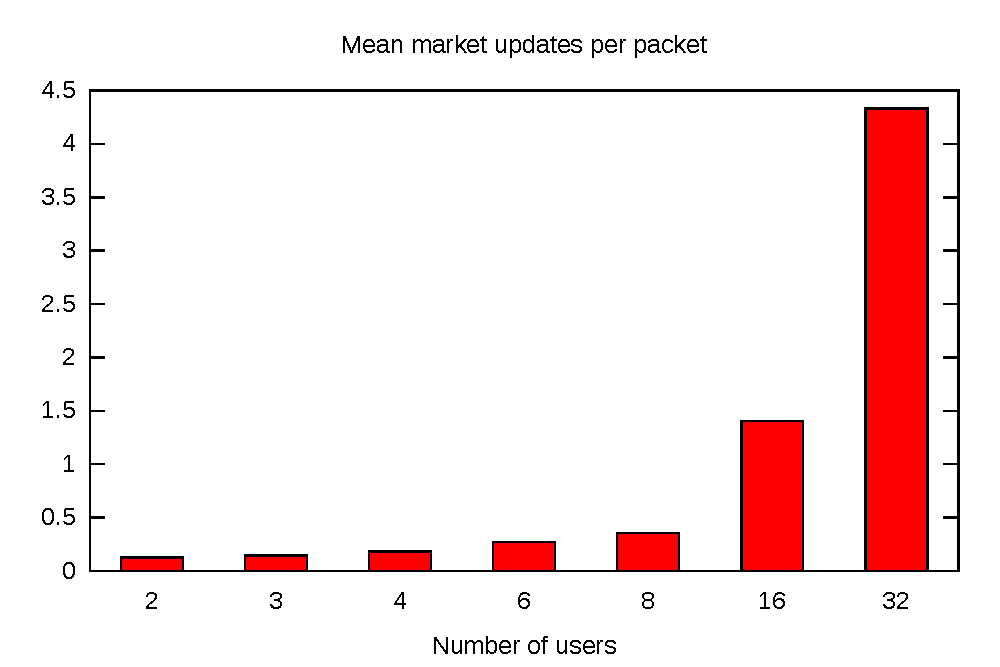
\includegraphics[width=\columnwidth]{plots/num_market_updates.pdf}
\caption{Mean number of sets of slot purchases made by flow completion time bots in simulation.}
\label{f:num_market_updates}
\end{figure}

Another problem with the simple market is that it can take a long time to converge on a solution where no user wants to buy more slots. In simulation, flow completion time user bots would buy back and forth from each other many times, making small price adjustments throughout.  
Figure~\ref{f:num_market_updates} shows the number times a user bought a set of packets on the market, or market updates, per packet sent in the simulations from in Figure~\ref{f:delay_over_srtf}.
More contention between slots increased the number of market updates required.

%TODO improve below sentence
The problems we encountered with the simple market led us to our current design:
\subsection{Multiresolution Market Design}

TODO

\begin{figure*}
\renewcommand{\arraystretch}{2}
\begin{tabular}[height=3in]{|*{8}{p{\slotwidth}|}}
\hline
\multicolumn{8}{|c|}{}\\
\hline
\multicolumn{4}{|c|}{} &\multicolumn{4}{c|}{} \\
\hline
\multicolumn{2}{|c|}{} &\multicolumn{2}{c|}{} &\multicolumn{2}{c|}{} &\multicolumn{2}{c|}{}\\
\hline
Time: 0 & Time: 1 & Time: 2 & Time: 3 & Time: 4 & Time: 5 & Time: 6 & Time: 7 \\
\{(A, \$2.01)\} & \{(A, \$2.01)\} & \{(B, )\} & \{(B, )\} & \{(ISP, \$1)\} & \{(ISP, \$1)\} & \{(C, \$10)\} & \{(ISP, \$1)\} \\
\hline
\end{tabular}
\caption{Multiresolution market order book.}
\label{f:multiresolution _market}
\end{figure*}
